\documentclass[11pt,a4paper]{article}
\usepackage[top=2.8cm,bottom=2.4cm,left=2.4cm,right=2.4cm,headheight=1.3cm,headsep=0.5cm]{geometry}
\usepackage{fontspec}
% Tipografias incluidas en TeX Live (funcionan en Overleaf sin instalar nada)
\setmainfont{TeX Gyre Heros}
\setsansfont{TeX Gyre Heros}
\setmonofont{Latin Modern Mono}
\usepackage{xcolor}
\definecolor{brandblue}{HTML}{1F4FB4}
\definecolor{brandgreen}{HTML}{2E9E5B}
\definecolor{ink}{HTML}{1B2236}
\definecolor{tintblue}{HTML}{E9EFFB}
\definecolor{tintgreen}{HTML}{E7F5EC}
\definecolor{greytext}{HTML}{5F6B7A}
% Alias de la identidad visual común (portada unificada)
\colorlet{gblue}{brandblue}
\colorlet{ggreen}{brandgreen}
\colorlet{gnavy}{ink}
\colorlet{ggray}{greytext}
\definecolor{gpale}{HTML}{8D919B}
\usepackage{graphicx,tikz,fancyhdr,titlesec,array,colortbl,setspace,needspace}
\usetikzlibrary{arrows.meta,positioning}
\usepackage[most]{tcolorbox}
\usepackage[colorlinks=true,linkcolor=brandblue,urlcolor=brandblue,pdftitle={Manual de coordinación – Los Gantt-sters},pdfauthor={Los Gantt-sters},pdfsubject={Manual de coordinación / Plan de dirección},pdflang={es}]{hyperref}

\renewcommand{\contentsname}{Índice}
\color{ink}
\setlength{\parindent}{0pt}
\setlength{\parskip}{0.7em}
\linespread{1.12}
\raggedright

% ---------- Cabecera y pie ----------
\pagestyle{fancy}
\fancyhf{}
\renewcommand{\headrulewidth}{0.6pt}
\renewcommand{\headrule}{{\color{brandblue}\hrule width\headwidth height\headrulewidth}}
\fancyhead[L]{\raisebox{-0.25cm}{
\includegraphics[height=0.95cm]{logo.png}}\hspace{0.3cm}{\small\bfseries\color{brandblue}LOS GANTT-STERS}}
\fancyhead[R]{\small\color{greytext}Manual de coordinación · Curso 2026-2027}
\fancyfoot[C]{{\color{brandgreen}\rule{2.6cm}{0.9pt}}\\[3pt]{\small\color{greytext}\thepage}}

% ---------- Títulos de sección ----------
\newcommand{\sectionbadge}[1]{\tikz[baseline=(n.base)]\node[fill=brandblue,text=white,rounded corners=3pt,inner xsep=5pt,inner ysep=3pt,minimum width=0.95cm](n){\bfseries #1};}
\titleformat{\section}{\Large\bfseries\color{brandblue}}{\sectionbadge{\thesection}}{0.7em}{}[\vspace{-0.1em}{\color{brandgreen}\titlerule[1.2pt]}]
\titleformat{name=\section,numberless}{\Large\bfseries\color{brandblue}}{}{0pt}{}[\vspace{-0.1em}{\color{brandgreen}\titlerule[1.2pt]}]
\titlespacing*{\section}{0pt}{1.5em}{0.9em}
\newcommand{\sectionbreak}{\needspace{7\baselineskip}}

% ---------- Utilidades ----------
\newcommand{\key}[1]{\textbf{\color{brandblue}#1}}
\tikzset{
 box/.style={rounded corners=4pt,draw=brandblue,fill=tintblue,text=ink,align=center,text width=3.1cm,minimum height=1.3cm,inner sep=5pt,font=\small},
 chip/.style={rounded corners=8pt,fill=tintgreen,draw=brandgreen,text=ink,align=center,inner xsep=9pt,inner ysep=3pt,font=\small\bfseries},
 arr/.style={-{Stealth[length=2.4mm]},brandgreen,line width=1.3pt}
}
\newcommand{\hdrcell}[1]{\cellcolor{brandblue}\textcolor{white}{\bfseries #1}}

\begin{document}

% ================= PORTADA (formato de la Propuesta técnica) =================
\begin{titlepage}
\centering
\vspace*{0.2cm}
{\fontsize{30}{34}\selectfont\bfseries\color{gblue}DGP\par}
\vspace{4pt}
{\small\bfseries\color{ggreen}Dirección y Gestión de Proyectos\par}
\vspace{0.8cm}

\includegraphics[width=4.2cm]{logo.png}\par
\vspace{0.9cm}
{\fontsize{24}{28}\selectfont\bfseries\color{gnavy}LOS GANTT-STERS\par}
\vspace{8pt}
{\color{ggreen}\rule{\linewidth}{1.2pt}\par}
\vspace{0.8cm}
{\fontsize{20}{24}\selectfont\bfseries\color{gblue}MANUAL DE COORDINACIÓN\par}
\vspace{6pt}
{\bfseries\color{gnavy}PLAN DE DIRECCIÓN\par}
\vspace{1.1cm}
{\footnotesize\bfseries\color{ggray}Integrantes\par}
\vspace{4pt}
{\color{gblue}\rule{\linewidth}{1.2pt}\par}
\vspace{10pt}
\begin{tabular}{c}
Javier Miñán Molina\\[3pt]
Germán Delgado Fernández\\[3pt]
Ana Meca Cano\\[3pt]
Jaime Montávez Ruiz\\[3pt]
Álvaro Sanabria Díaz\\[3pt]
Juan Luis Jiménez Urbano
\end{tabular}\par
\vspace{14pt}
{\small\color{gpale}Universidad de Granada · Curso 2026-2027\par}
\end{titlepage}

% ================= PRESENTACIÓN =================
\vspace{0.2em}
{\setlength{\parskip}{0pt}\renewcommand{\arraystretch}{1.6}\arrayrulecolor{brandblue!35}
\begin{tabular}{@{}>{\bfseries\color{brandblue}\hbox to 3.6cm\bgroup}l<{\hfil\egroup}p{11.6cm}@{}}
Proyecto & Agenda personalizada accesible para estudiantes con discapacidad intelectual \\ \hline
Cliente & Colegio de Educación Especial Fundación Purísima Concepción (Granada) \\ \hline
Grupo & Los Gantt-sters \\ \hline
Fecha & 08/10/2026 \\ \hline
\end{tabular}}

\vspace{0.6em}
{\large\bfseries\color{brandgreen}El proyecto de un vistazo}\par
\vspace{0.2em}
{\setlength{\parskip}{0pt}\renewcommand{\arraystretch}{1.6}\rowcolors{1}{tintblue}{white}\arrayrulecolor{white}
\begin{tabular}{@{\hspace{6pt}}>{\bfseries\color{brandblue}\hbox to 5.2cm\bgroup}l<{\hfil\egroup}p{9.8cm}@{}}
Metodología & Scrum, con estimación del trabajo de cada iteración \\
Gestión de los sprints & Jira \\
Plataforma & Aplicación web (webapp), con prioridad a tablets en formato horizontal \\
Framework e IDE & Native para el front-end y VSCode \\
Backend y hosting & Supabase y Vercel \\
Código & GitHub, con \texttt{master} como rama del trabajo definitivo \\
Documentación compartida & Google Drive \\
Documentación técnica & LaTeX, con identidad visual común \\
Comunicación & WhatsApp, videollamadas y reuniones periódicas \\
Seguimiento & Reunión semanal como mínimo con el profesorado \\
Desempeño & Trabajo asignado por iteración; mínimo del 75 \% para no acumular carga \\
Plazo interno & Todo finalizado y listo dos días antes de la entrega oficial \\
\end{tabular}}

% ================= SECCIONES =================
\clearpage
\section{Metodología de desarrollo y ciclo de vida}
Para la gestión técnica del proyecto se empleará la metodología ágil \key{Scrum}. Inicialmente se realizará una definición completa de los requisitos de la aplicación y se asignarán los roles de cada componente del grupo. Además, se llevará a cabo una estimación del trabajo que deberá realizarse en cada una de las iteraciones.

Para organizar Scrum y los sprints se utilizará la aplicación \key{Jira}. En ella se mantendrá el Product Backlog con sus épicas e historias de usuario, se planificará cada sprint, se repartirán las tareas entre los miembros del equipo y se seguirá su avance en el tablero del sprint.

\section{Recursos software de desarrollo}
El desarrollo se realizará utilizando lenguajes y herramientas de uso libre o con licencia universitaria. Todo el proyecto se desarrollará como una \key{aplicación web} (webapp), que se usa desde el navegador y se orienta en primer lugar a tablets en formato horizontal. Concretamente, se empleará \key{Native} para desarrollar el front-end, \key{Supabase} como backend y \key{Vercel} para publicar la aplicación, con \key{VSCode} como entorno de desarrollo integrado (IDE). La gestión y control del código se centralizará en \key{GitHub}. Los sprints se organizarán en \key{Jira}. Para la documentación compartida se utilizará \key{Google Drive}, y la comunicación diaria del equipo se canalizará mediante \key{WhatsApp}.

\section{Organización del equipo de trabajo (estructura, normas)}
La asignación inicial de roles y tareas se realizará por decisión unánime del equipo. Se establecen normas y estándares de trabajo de obligado cumplimiento: al inicio de cada iteración se asignará un trabajo a cada persona y, si un miembro del equipo no completa al menos el \key{75\,\%} del trabajo que se le asignó, su carga de trabajo se incrementará en la iteración siguiente con la carga pendiente. Asimismo, como norma general, todos los trabajos deberán estar finalizados y listos \key{dos días antes} de la fecha de entrega oficial.

\section{Herramientas para comunicaciones en el equipo de trabajo}
Las comunicaciones asíncronas se realizarán a través de un grupo de trabajo específico en \key{WhatsApp}, proporcionando información de forma ágil y centralizada. Esta vía se complementará con videollamadas cuando sea necesario, reuniones periódicas planificadas y tiempo de trabajo conjunto durante las clases prácticas.

\section{Relaciones con el cliente (entrevistas, reuniones, revisiones, \ldots)}
Al menos una vez a la semana se mantendrán reuniones de seguimiento con el profesorado encargado para consultar dudas, plantear inquietudes y reportar el estado del trabajo. La comunicación directa con el cliente se gestionará siguiendo estrictamente las directrices del profesorado y se adaptará a las necesidades específicas de supervisión del proyecto.

\section{Estándares de documentación}
Todos los documentos generados compartirán una misma identidad visual (portada, estructura, tipografía y logotipo). Para facilitar la estandarización y asegurar la calidad del formato, la adecuación y la corrección, toda la documentación técnica se redactará utilizando \key{LaTeX}.

\section{Estándares de código}
Se exigirá un código limpio e inteligible, siendo obligatorio el uso de comentarios explicativos en las partes esenciales del código. Además, se deberán incluir cabeceras descriptivas en todas las funciones y utilizar nomenclaturas claras y representativas para las variables.

\section{Plan de gestión de cambios}
Ante cualquier solicitud de cambio (ya sea por prevención, reparación o mejora), el coordinador deberá convocar una reunión específica. En ella se concretará qué elementos deben modificarse, se analizarán sus implicaciones y se adaptarán las tareas previstas redistribuyendo el trabajo entre el equipo.

\begin{center}
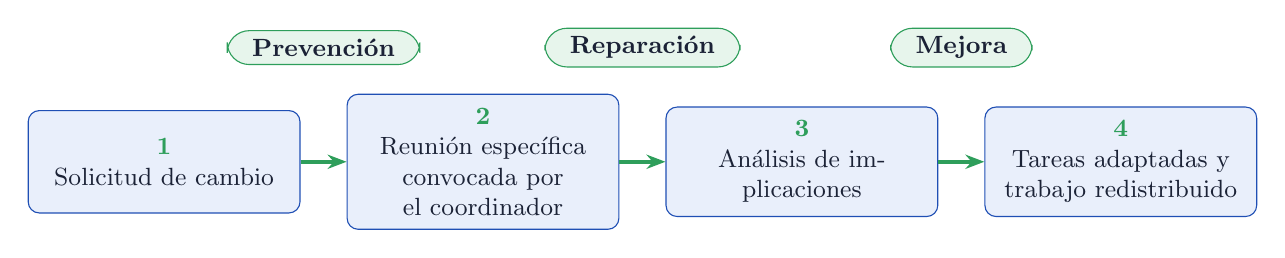
\begin{tikzpicture}
\node[chip] at (-4.05,1.45) {Prevención};
\node[chip] at (0,1.45) {Reparación};
\node[chip] at (4.05,1.45) {Mejora};
\node[box](a) at (-6.075,0) {\textbf{\color{brandgreen}1}\\Solicitud de cambio};
\node[box](b) at (-2.025,0) {\textbf{\color{brandgreen}2}\\Reunión específica convocada por el coordinador};
\node[box](c) at (2.025,0) {\textbf{\color{brandgreen}3}\\Análisis de implicaciones};
\node[box](d) at (6.075,0) {\textbf{\color{brandgreen}4}\\Tareas adaptadas y trabajo redistribuido};
\draw[arr](a)--(b); \draw[arr](b)--(c); \draw[arr](c)--(d);
\end{tikzpicture}
\end{center}

\section{Control de versiones (método y herramientas)}
Se mantendrá un control de versiones adecuado utilizando repositorios en \key{GitHub}. El flujo de trabajo establecerá que cada persona clonará la rama principal (\texttt{master}, que representa el trabajo definitivo) para desarrollar sus tareas. Una vez que la funcionalidad esté perfectamente implementada, el gestor de calidad revisará el trabajo en esa rama paralela y, si aprueba su corrección, procederá a integrar (fusionar) el código en la rama \texttt{master}.

\begin{center}
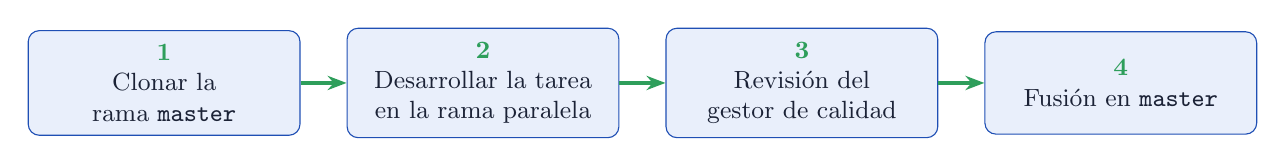
\begin{tikzpicture}
\node[box](a) at (-6.075,0) {\textbf{\color{brandgreen}1}\\Clonar la rama \texttt{master}};
\node[box](b) at (-2.025,0) {\textbf{\color{brandgreen}2}\\Desarrollar la tarea en la rama paralela};
\node[box](c) at (2.025,0) {\textbf{\color{brandgreen}3}\\Revisión del gestor de calidad};
\node[box](d) at (6.075,0) {\textbf{\color{brandgreen}4}\\Fusión en \texttt{master}};
\draw[arr](a)--(b); \draw[arr](b)--(c); \draw[arr](c)--(d);
\end{tikzpicture}
\end{center}

\section{Gestión de calidad (durante el desarrollo y al final, incluir herramientas)}
El gestor de calidad será el encargado de revisar el trabajo y garantizar su nivel antes de cada entrega. Esta figura deberá coordinarse estrechamente con el miembro encargado de auditar la usabilidad y la accesibilidad para comprobar que el producto cumple con los estándares exigidos. En caso de detectar errores, el gestor de calidad se comunicará con el coordinador para que este asigne la tarea de corrección al integrante correspondiente. Como herramientas se emplearán \key{GitHub} (revisión de ramas), \texttt{ESLint} y \texttt{Prettier} para el código, listas de comprobación para documentos y código, y un registro de no conformidades. El código del gestor de calidad será revisado por el gestor de usabilidad y accesibilidad. Al final del proyecto se redactará un informe de calidad con los resultados, indicadores y no conformidades.

\section{Plan de medición del desempeño, recompensas}
El desempeño de los miembros se medirá a través de un plan de objetivos personales por iteración, evaluando el cumplimiento estricto de la planificación. Al inicio de cada iteración se asignará su trabajo a cada persona en \key{Jira} y, al finalizarla, se verificará el porcentaje de trabajo completado por cada individuo. Si una persona finaliza menos del \key{75\,\%} de las tareas que tenía asignadas, la carga pendiente se le acumulará como penalización para la iteración siguiente.


\end{document}
